\chapter{Statistical Models and Maximum Likelihood Estimation}

\section{Statistical models}

Data vary from unit to unit and from sample to sample. A \emph{statistical model}
describes this variability with a probability distribution: we regard the observed data
$y_1,\dots,y_n$ as realizations of random variables $Y_1,\dots,Y_n$ whose distribution
depends on unknown \emph{parameters} $\theta$ (possibly a vector). Parameters are linked
to the attributes we care about (e.g.\ $\theta$ = proportion of voters supporting a party).

\begin{remark}[Notation]
Capital letters $Y$ are random variables; lower case $y$ are observed values. An
\emph{estimate} $\thetahat$ is a number computed from $y$; the corresponding
\emph{estimator} $\tilde\theta$ is the same function applied to the random $Y$.
\end{remark}

\subsection{Choosing a model}
Model choice is guided by
\begin{itemize}
  \item \textbf{background knowledge} of the process: a count of successes in $n$
        independent trials suggests $\Bin(n,\theta)$; counts of rare events in time or
        space suggest $\Poi(\theta)$; waiting times between events in a Poisson process
        suggest $\Expo(\theta)$; measurements that are sums of many small effects
        suggest $\Gau(\mu,\sigma)$;
  \item \textbf{past experience} with similar data;
  \item \textbf{the data themselves}: histograms, ECDFs and QQ plots (Chapter 1).
\end{itemize}
``All models are wrong, but some are useful'': a model is an approximation that should be
good enough for the question at hand. In these notes $\Gau(\mu,\sigma)$ denotes the Gaussian
(normal) distribution with mean $\mu$ and \emph{standard deviation} $\sigma$.

\begin{center}
\begin{tabular}{llll}
\toprule
Model & p.f./p.d.f.\ & Mean & Variance \\
\midrule
$\Bin(n,\theta)$ & $\binom{n}{y}\theta^y(1-\theta)^{n-y}$, $y=0,\dots,n$ & $n\theta$ & $n\theta(1-\theta)$\\
$\Poi(\theta)$ & $\theta^y e^{-\theta}/y!$, $y=0,1,\dots$ & $\theta$ & $\theta$ \\
$\Expo(\theta)$ & $\frac1\theta e^{-y/\theta}$, $y>0$ & $\theta$ & $\theta^2$ \\
$\Gau(\mu,\sigma)$ & $\frac{1}{\sqrt{2\pi}\sigma}e^{-(y-\mu)^2/(2\sigma^2)}$ & $\mu$ & $\sigma^2$\\
\bottomrule
\end{tabular}
\end{center}

\section{The likelihood function}

\begin{definition}[Likelihood]
Suppose the data $y$ have probability (density) function $f(y;\theta)$. The
\emph{likelihood function} is
\[
L(\theta) = L(\theta; y) = c \cdot \Prob(\text{observing the data } y;\ \theta),
\qquad \theta\in\Omega,
\]
viewed as a function of $\theta$ with $y$ fixed; $c$ is any positive constant not depending
on $\theta$. For independent observations $y_1,\dots,y_n$,
$L(\theta) = \prod_{i=1}^n f(y_i;\theta)$. For continuous data we use the p.d.f.\ (which is
proportional to the probability of observing a value in a small interval around $y_i$).
\end{definition}

\begin{definition}[MLE, log-likelihood, relative likelihood]
\begin{itemize}
  \item The \emph{maximum likelihood estimate} (MLE) $\thetahat$ is the value of $\theta$
        that maximizes $L(\theta)$: the parameter value that makes the observed data most
        probable.
  \item The \emph{log-likelihood} is $\ell(\theta) = \log L(\theta)$ (natural log). Since
        $\log$ is increasing, $\ell$ and $L$ have the same maximizer, and $\ell$ turns
        products into sums. Usually we solve the \emph{score equation}
        $\ell'(\theta) = 0$ and check it is a maximum.
  \item The \emph{relative likelihood} is $R(\theta) = L(\theta)/L(\thetahat)$, so
        $0\le R(\theta)\le 1$ and $R(\thetahat)=1$. It measures how plausible $\theta$ is
        compared with the best value, and is free of the arbitrary constant $c$.
\end{itemize}
\end{definition}

\begin{remark}
If two independent studies give data $y^{(1)}$ and $y^{(2)}$ about the same $\theta$, the
combined likelihood is the product $L_1(\theta)L_2(\theta)$ (log-likelihoods add).
\end{remark}

\section{MLEs for standard models}

\begin{theorem}[Binomial]
If $Y\sim\Bin(n,\theta)$ and we observe $y$, then $\thetahat = y/n$.
\end{theorem}
\begin{proof}
$L(\theta) = \theta^y(1-\theta)^{n-y}$ (dropping $\binom ny$), so
$\ell(\theta) = y\log\theta + (n-y)\log(1-\theta)$ and
$\ell'(\theta) = \frac{y}{\theta} - \frac{n-y}{1-\theta}$. Setting this to $0$ gives
$y(1-\theta) = (n-y)\theta$, i.e.\ $\theta = y/n$. Since
$\ell''(\theta) = -y/\theta^2 - (n-y)/(1-\theta)^2 < 0$, it is a maximum (for $0<y<n$;
the boundary cases give $\thetahat=0$ or $1$ directly).
\end{proof}

\begin{theorem}[Poisson]
If $Y_1,\dots,Y_n$ are independent $\Poi(\theta)$, then $\thetahat = \ybar$.
\end{theorem}
\begin{proof}
$L(\theta) = \prod \theta^{y_i}e^{-\theta}/y_i! \propto \theta^{\sum y_i} e^{-n\theta}$, so
$\ell(\theta) = \big(\sum y_i\big)\log\theta - n\theta$ and
$\ell'(\theta) = \sum y_i/\theta - n = 0$ gives $\thetahat = \ybar$; $\ell''<0$.
\end{proof}

\begin{theorem}[Exponential]
If $Y_1,\dots,Y_n$ are independent $\Expo(\theta)$ (mean $\theta$), then $\thetahat=\ybar$.
\end{theorem}
\begin{proof}
$L(\theta) = \theta^{-n}e^{-\sum y_i/\theta}$, $\ell(\theta) = -n\log\theta - \sum
y_i/\theta$, $\ell'(\theta) = -n/\theta + \sum y_i/\theta^2 = 0 \iff \theta = \ybar$.
\end{proof}

\begin{theorem}[Gaussian]
If $Y_1,\dots,Y_n$ are independent $\Gau(\mu,\sigma)$ with both parameters unknown, then
\[
\hat\mu = \ybar, \qquad \hat\sigma^2 = \frac1n\sum_{i=1}^n (y_i-\ybar)^2.
\]
\end{theorem}
\begin{proof}
$\ell(\mu,\sigma) = -n\log\sigma - \frac{1}{2\sigma^2}\sum (y_i-\mu)^2$ (plus a
constant). Then
$\partial\ell/\partial\mu = \frac{1}{\sigma^2}\sum(y_i-\mu) = 0$ gives $\hat\mu=\ybar$ for
every $\sigma$, and
$\partial\ell/\partial\sigma = -\frac n\sigma + \frac{1}{\sigma^3}\sum(y_i-\mu)^2 = 0$
gives $\hat\sigma^2 = \frac1n\sum(y_i-\ybar)^2$.
\end{proof}

Note that the Gaussian MLE of $\sigma^2$ divides by $n$, whereas the sample variance $s^2$
divides by $n-1$. For large $n$ the difference is negligible.

\section{Worked examples}

\begin{example}[Binomial survey]
\label{ex:binsurvey}
In a random sample of $n=200$ students, $y=58$ say they work part time. Model:
$Y\sim\Bin(200,\theta)$. Then $\thetahat = 58/200 = 0.29$ and
\[
\ell(\theta) = 58\log\theta + 142\log(1-\theta), \qquad
R(\theta) = \left(\frac{\theta}{0.29}\right)^{58}\left(\frac{1-\theta}{0.71}\right)^{142}.
\]
For instance $R(0.25) = 0.438$ and $R(0.35) = 0.196$: $\theta=0.25$ is quite plausible,
$\theta=0.35$ less so. Solving $R(\theta) = 0.1$ numerically gives
$\theta \approx 0.225$ and $0.362$ (this will be a \emph{10\% likelihood interval},
Chapter 4).
\begin{center}
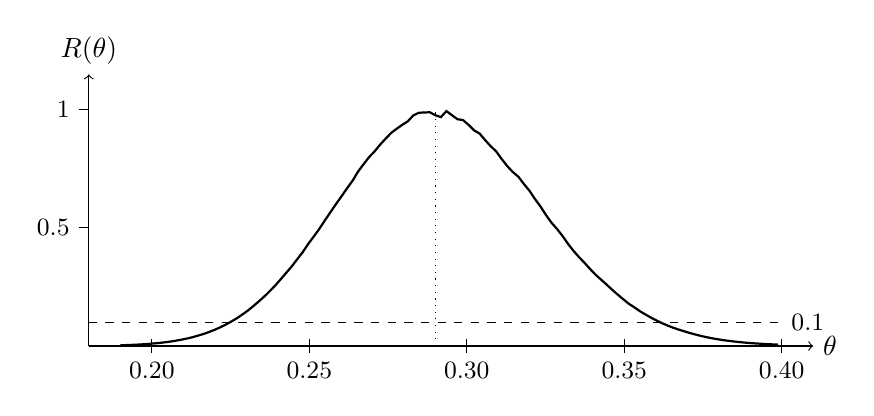
\begin{tikzpicture}[x=40cm,y=3cm]
  \draw[->] (0.18,0) -- (0.41,0) node[right] {$\theta$};
  \draw[->] (0.18,0) -- (0.18,1.15) node[above] {$R(\theta)$};
  \foreach \t in {0.20,0.25,0.30,0.35,0.40} \draw (\t,0.03) -- (\t,-0.03) node[below] {\small \t};
  \foreach \r in {0.5,1} \draw (0.18,\r) -- (0.177,\r) node[left] {\small \r};
  \draw[thick,domain=0.19:0.40,samples=120] plot (\x,{exp(58*ln(\x/0.29)+142*ln((1-\x)/0.71))});
  \draw[dashed] (0.18,0.1) -- (0.40,0.1) node[right] {\small $0.1$};
  \draw[dotted] (0.29,0) -- (0.29,1);
\end{tikzpicture}
\end{center}
\end{example}


\begin{center}
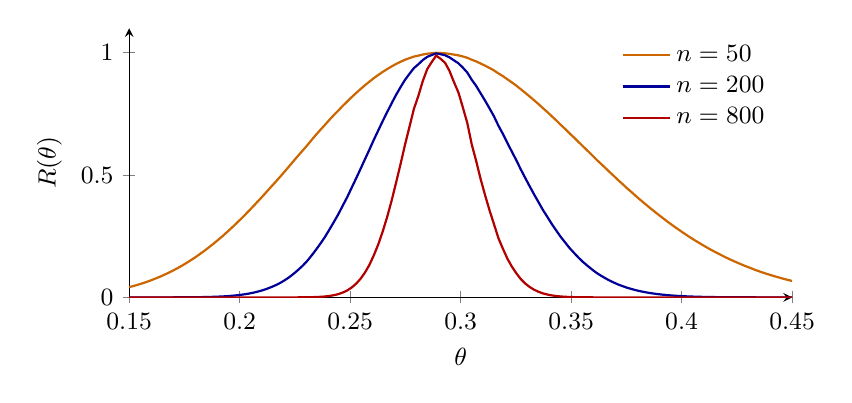
\begin{tikzpicture}
\begin{axis}[width=10cm, height=5cm, xmin=0.15, xmax=0.45, ymin=0, ymax=1.1, xlabel={$\theta$},
    ylabel={$R(\theta)$}, tick label style={font=\small}, label style={font=\small}, axis lines=left, scaled y ticks=false, yticklabel style={/pgf/number format/fixed}, samples=150, xticklabel style={/pgf/number format/fixed},
    legend style={font=\small, draw=none}, legend cell align=left]
  \addplot[thick, orange!80!black, domain=0.15:0.45] {exp(14.499999999999998*ln(x/0.29)+35.5*ln((1-x)/0.71))};
  \addplot[thick, blue!60!black, domain=0.15:0.45] {exp(57.99999999999999*ln(x/0.29)+142.0*ln((1-x)/0.71))};
  \addplot[thick, red!70!black, domain=0.15:0.45] {exp(231.99999999999997*ln(x/0.29)+568.0*ln((1-x)/0.71))};
  \legend{$n=50$, $n=200$, $n=800$}
\end{axis}
\end{tikzpicture}
\end{center}
With the same sample proportion $0.29$, larger samples give a narrower relative likelihood:
more data rule out more values of $\theta$.

\begin{example}[Poisson counts and invariance]
The numbers of help-desk calls in $10$ randomly chosen five-minute periods were
$3,5,2,4,6,1,3,4,2,5$. Assuming independent $\Poi(\theta)$ counts, $\sum y_i = 35$ and
$\thetahat = 35/10 = 3.5$ calls per period. The relative likelihood is
$R(\theta) = (\theta/3.5)^{35}e^{10(3.5-\theta)}$.
\end{example}

\begin{center}
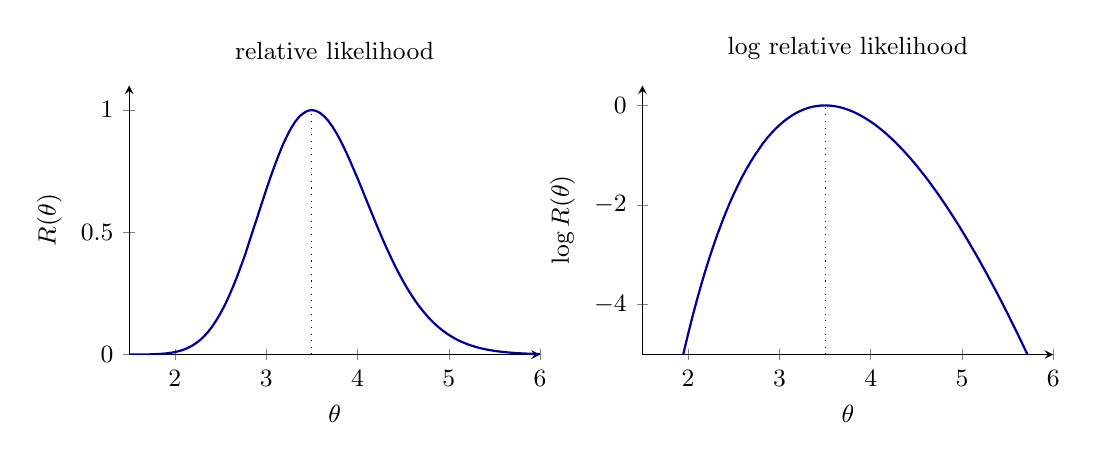
\begin{tikzpicture}
\begin{axis}[name=r1, width=6.8cm, height=5cm, xmin=1.5, xmax=6, ymin=0, ymax=1.1, xlabel={$\theta$},
    ylabel={$R(\theta)$}, tick label style={font=\small}, label style={font=\small}, axis lines=left, scaled y ticks=false, yticklabel style={/pgf/number format/fixed}, samples=100, title={relative likelihood}, title style={font=\small}]
  \addplot[thick, blue!60!black, domain=1.5:6] {exp(35*ln(x/3.5)+10*(3.5-x))};
  \draw[dotted] (axis cs:3.5,0) -- (axis cs:3.5,1);
\end{axis}
\begin{axis}[at={(r1.east)}, anchor=west, xshift=1.3cm, width=6.8cm, height=5cm, xmin=1.5, xmax=6,
    ymin=-5, ymax=0.4, xlabel={$\theta$}, ylabel={$\log R(\theta)$}, tick label style={font=\small}, label style={font=\small}, axis lines=left, scaled y ticks=false, yticklabel style={/pgf/number format/fixed}, samples=100,
    title={log relative likelihood}, title style={font=\small}]
  \addplot[thick, blue!60!black, domain=1.5:6] {35*ln(x/3.5)+10*(3.5-x)};
  \draw[dotted] (axis cs:3.5,-5) -- (axis cs:3.5,0);
\end{axis}
\end{tikzpicture}
\end{center}
Both curves peak at $\thetahat = 3.5$ (dotted). Taking logs turns the product of $10$
Poisson probabilities into a sum and makes the curve close to a parabola near its maximum.

\begin{theorem}[Invariance property]
If $\thetahat$ is the MLE of $\theta$ and $\tau = h(\theta)$, then the MLE of $\tau$ is
$\hat\tau = h(\thetahat)$.
\end{theorem}
\begin{proof}[Proof sketch]
For one-to-one $h$, $L$ expressed in terms of $\tau$ is $L(h^{-1}(\tau))$, which is
maximized when $h^{-1}(\tau) = \thetahat$. For general $h$ one defines the induced
likelihood $L^*(\tau) = \sup_{\theta: h(\theta)=\tau} L(\theta)$, which is maximized at
$\tau=h(\thetahat)$.
\end{proof}

\begin{example}[Using invariance]
\begin{itemize}
  \item Poisson calls: the MLE of $\Prob(Y=0) = e^{-\theta}$ is $e^{-3.5} = 0.0302$, and
        of $\Prob(Y\le 1) = e^{-\theta}(1+\theta)$ is $e^{-3.5}(4.5) = 0.1359$.
  \item Exponential lifetimes (in years) of $8$ components:
        $2.1,0.4,5.3,1.8,3.6,0.9,7.2,2.7$. Then $\sum y_i = 24.0$, $\thetahat = 3.0$. The
        MLE of $\Prob(Y>5) = e^{-5/\theta}$ is $e^{-5/3} = 0.1889$, and of the median
        lifetime $\theta\log 2$ is $3\log 2 = 2.079$ years.
  \item Gaussian: from $n=10$ fill weights (grams)
        $12.4,11.8,13.1,12.9,12.0,13.5,12.7,11.6,12.2,13.0$ we get $\sum y_i = 125.2$,
        $\sum y_i^2 = 1570.96$, so $\hat\mu = 12.52$,
        $S_{yy} = 1570.96 - 125.2^2/10 = 3.456$, $\hat\sigma^2 = 0.3456$, and by invariance
        $\hat\sigma = \sqrt{0.3456} = 0.5879$. (By contrast, $s = \sqrt{3.456/9} = 0.6197$.)
\end{itemize}
\end{example}

\section{Checking the model}

After fitting, ask whether the model is consistent with the data:
\begin{enumerate}
  \item \textbf{Observed vs expected frequencies.} For discrete data (or grouped
        continuous data), compare the observed count in each class with the expected count
        $n\,\hat p_j$ computed from the fitted model. (Chapter 7 turns this into a formal
        test.)
  \item \textbf{Graphs.} Superimpose the fitted p.d.f.\ on a relative frequency histogram,
        or the fitted c.d.f.\ on the ECDF; use a Gaussian QQ plot for Gaussian models.
  \item \textbf{Summary statistics.} E.g.\ for a Poisson model the sample mean and sample
        variance should be similar; for an exponential model the sample mean and sample
        standard deviation should be similar; for a Gaussian model skewness $\approx 0$
        and kurtosis $\approx 3$.
\end{enumerate}

\begin{example}[Observed vs expected under a Poisson fit]
In $200$ one-minute intervals the numbers of cars passing a point were recorded:
\begin{center}
\begin{tabular}{lccccc}
\toprule
cars & $0$ & $1$ & $2$ & $3$ & $\ge 4$ \\
\midrule
observed & 38 & 80 & 50 & 20 & 12 \\
\bottomrule
\end{tabular}
\end{center}
The $12$ intervals in the last class had $9$ fours and $3$ fives, so the total count is
$80 + 2(50) + 3(20) + 4(9) + 5(3) = 291$ and $\thetahat = 291/200 = 1.455$. The fitted
probabilities $e^{-1.455}1.455^y/y!$ for $y=0,1,2,3$ are $0.2334, 0.3396, 0.2471,
0.1198$, and $\Prob(Y\ge4) = 0.0601$. Expected frequencies (multiply by $200$):
$46.68, 67.92, 49.41, 23.96, 12.02$. The agreement is reasonable, with somewhat fewer
zeros and more ones than the model predicts; Chapter 7 shows that this discrepancy is
well within chance variation.
\end{example}

\begin{center}
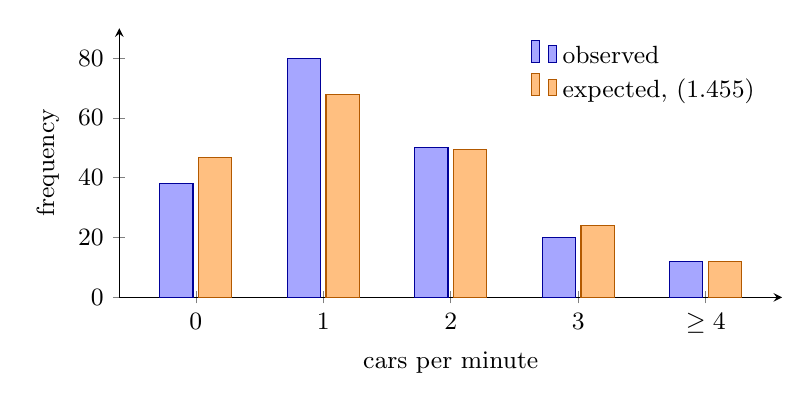
\begin{tikzpicture}
\begin{axis}[width=10cm, height=5cm, ybar, bar width=12pt, ymin=0, ymax=90, xtick={0,1,2,3,4},
    xticklabels={$0$,$1$,$2$,$3$,$\ge4$}, xlabel={cars per minute}, ylabel={frequency}, tick label style={font=\small}, label style={font=\small}, axis lines=left, scaled y ticks=false, yticklabel style={/pgf/number format/fixed},
    enlarge x limits=0.15, legend style={font=\small, draw=none}, legend cell align=left]
  \addplot[fill=blue!35, draw=blue!60!black] coordinates {(0,38) (1,80) (2,50) (3,20) (4,12)};
  \addplot[fill=orange!50, draw=orange!70!black] coordinates {(0,46.68) (1,67.92) (2,49.41) (3,23.96) (4,12.02)};
  \legend{observed, {expected, $\Poi(1.455)$}}
\end{axis}
\end{tikzpicture}
\end{center}

\begin{important}[Common pitfalls]
\begin{itemize}
  \item The likelihood is a function of $\theta$, not a probability distribution for
        $\theta$: it need not integrate to $1$.
  \item Do not forget to check that a stationary point is a maximum, and watch for
        boundary maxima (e.g.\ $y=0$ in the binomial).
  \item Parametrization matters for writing formulas: our exponential has
        \emph{mean} $\theta$ (rate $1/\theta$), and $\Gau(\mu,\sigma)$ uses the standard
        deviation.
\end{itemize}
\end{important}

\section*{Summary}
\begin{itemize}
  \item $L(\theta) \propto \Prob(\text{data};\theta)$; $\ell = \log L$;
        $R(\theta) = L(\theta)/L(\thetahat)\in[0,1]$.
  \item MLEs: binomial $y/n$; Poisson $\ybar$; exponential $\ybar$; Gaussian
        $\hat\mu=\ybar$, $\hat\sigma^2 = \frac1n\sum(y_i-\ybar)^2$.
  \item Invariance: the MLE of $h(\theta)$ is $h(\thetahat)$.
  \item Check fit with observed vs expected frequencies, plots and summary statistics.
\end{itemize}
